\documentclass[10pt]{article}
\usepackage{babel}
\usepackage[utf8]{inputenc}
\usepackage[T1]{fontenc}
\usepackage{graphicx}
\usepackage[export]{adjustbox}
\graphicspath{ {./images/} }
\usepackage{amsmath}
\usepackage{amsfonts}
\usepackage{amssymb}
\usepackage[version=4]{mhchem}
\usepackage{stmaryrd}

\begin{document}
\section*{1. Introducción y objetivos del experimento}
El presente informe se basa en los datos recopilados de la experimentación en el laboratorio de Física II, en la Facultad de Ciencias. Se apoya en la guía de laboratorio y otras fuentes detalladas más adelante. El propósito del informe es responder las preguntas del cuestionario, de manera adecuada; así como contrastar los resultados de la experimentación con el fundamento teórico. De acuerdo a la guía del laboratorio e indicaciones del profesor, se ha dividido el informe de la siguiente manera.

\subsection*{1.1. Contenido}
\begin{enumerate}
  \item Introducción y objetivos del experimento
\end{enumerate}

\begin{itemize}
  \item Contenido
  \item Competencias generales
\end{itemize}

\begin{enumerate}
  \setcounter{enumi}{1}
  \item Fundamento teórico
\end{enumerate}

\begin{itemize}
  \item Esfuerzo, deformación y módulos de elasticidad
  \item Esfuerzo y deformación de tensión y compresión
  \item Esfuerzo y deformación volumétrico
  \item Esfuerzo y deformación por corte
  \item Deformaciones transversales
  \item Elasticidad y plasticidad
  \item Histéresis elástica
  \item Aplicaciones al experimento
\end{itemize}

\begin{enumerate}
  \setcounter{enumi}{2}
  \item Equipo utilizado y diagrama de flujo del experimento
\end{enumerate}

\begin{itemize}
  \item Equipo utilizado
  \item Diagrama de flujo del experimento
\end{itemize}

\begin{enumerate}
  \setcounter{enumi}{3}
  \item Procedimiento experimental
  \item Cálculos y resultados
\end{enumerate}

\begin{itemize}
  \item Uso de unidades
  \item Uso de cifras significativas
  \item Cálculo de errores
  \item Resultados obtenidos y comparación con otros conocidos
  \item Tablas, gráficos y comparación con otros resultados conocidos
\end{itemize}

\begin{enumerate}
  \setcounter{enumi}{5}
  \item Cuestionario, observaciones y sugerencias
\end{enumerate}

\begin{itemize}
  \item Respuestas al cuestionario
  \item Observaciones
  \item Sugerencias
\end{itemize}

\begin{enumerate}
  \setcounter{enumi}{6}
  \item Conclusiones
  \item Bibliografía
\end{enumerate}

\subsection*{1.2. Competencias generales}
\begin{itemize}
  \item Hallar experimentalmente la relación entre el esfuerzo aplicado y la deformación unitaria bajo condiciones de elasticidad.\\
*Aclaración: Debido a indicaciones del profesor, se usó otra tabla en lugar de la que está en la guía.
\end{itemize}

\section*{2. Fundamento teórico}
\subsection*{2.1. Esfuerzo, deformación y módulos de elasticidad}
En muchos casos, los procesos de estiramiento, compresión, flexión, torcedura y corte de los cuerpos reales son muy importante, por lo que no pueden ser despreciables.\\
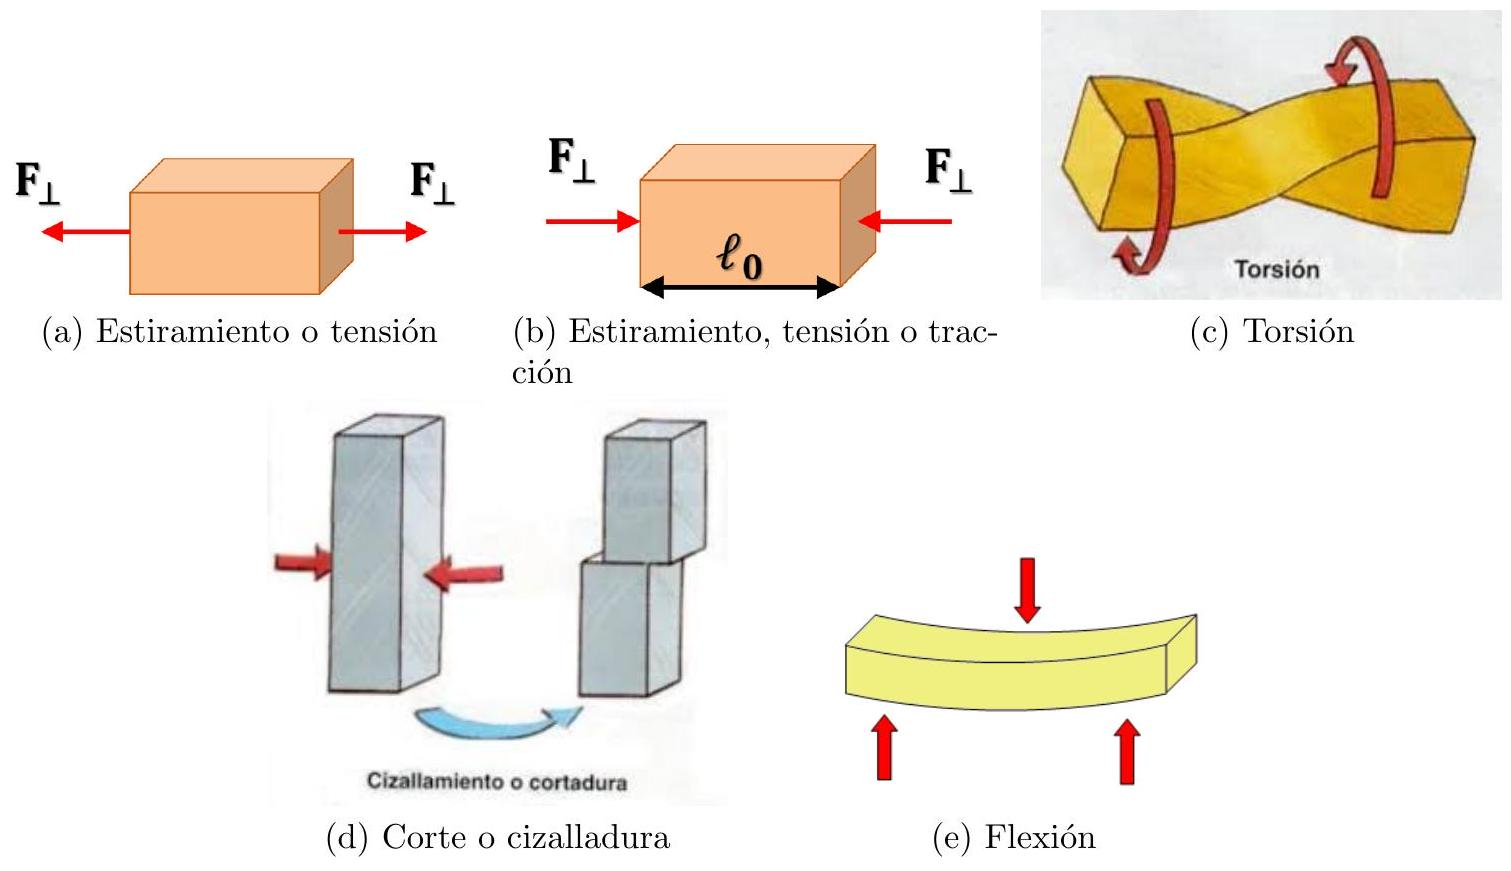
\includegraphics[max width=\textwidth, center]{2025_04_28_a9941da8947ada55c6c9g-02}

Todo cuerpo sólido se deforma bajo la acción de fuerzas, y al cesar estas, tiende a recuperar su forma, esta tendencia se denomina elasticidad. En la realidad, no hay cuerpo perfectamente elástico o inelástico, solo cuerpo con deformaciones con parte elástica y permanente. Generalmente, si las fuerzas no sobrepasan determinados valores, los cuerpos pueden considerarse elásticos.

\subsection*{2.1.1. Módulo de elasticidad}
Para cada clase de deformación, se introducen las cantidades esfuerzo( $\sigma$ )(intensidad de fuerzas que causan la deformación) y deformación unitaria( $(\varepsilon)$ (cambio de forma resultante). Si tenemos esfuerzo y deformación unitaria pequeños, podemos establecer que son directamente proporcionales(comprobado experimentalmente). Luego, dentro de este intervalo, definimos al módulo de elasticidad $(M)$ como :


\begin{equation*}
M=\frac{\sigma}{\varepsilon} \tag{1}
\end{equation*}


A este comportamiento se le denomina"Ley de Hooke".

\subsection*{2.2. Esfuerzo y deformación de tensión y compresión}
\subsection*{2.2.1. Esfuerzo y deformación por tensión}
Cuando un cuerpo se somete a fuerzas que tiran de sus extremos, tiende a incrementar su longitud respecto a la dirección de estas fuerzas; en el caso de una barra tenemos:\\
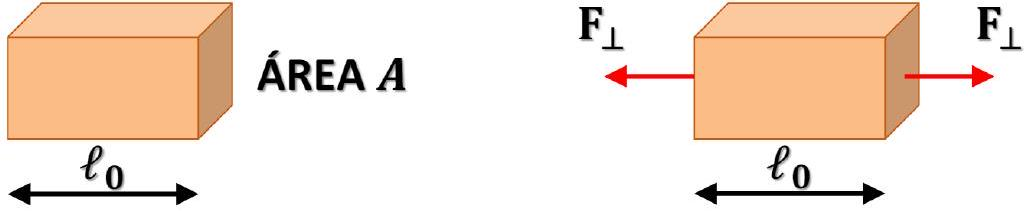
\includegraphics[max width=\textwidth, center]{2025_04_28_a9941da8947ada55c6c9g-03(1)}

Figura 1: Estiramiento de barra\\
Definimos al esfuerzo de tensión $(\sigma)$ como cociente entre fuerza $\left(F_{\perp}\right)$ y área transversal $(A)$ :


\begin{equation*}
\sigma=\frac{F_{\perp}}{A} \tag{2}
\end{equation*}


Cantidad escalar, puesto que solo abajamos con la intensidad de la fuerza $\left(\frac{N}{m^{2}}\right)(P a)$.\\
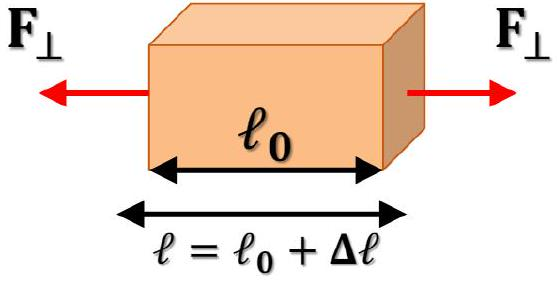
\includegraphics[max width=\textwidth, center]{2025_04_28_a9941da8947ada55c6c9g-03}

Figura 2: Longitud final de barra\\
Sea $\ell_{0}$ la longitud inicial y $\ell$ la longitud final, tenemos que la variación de longitud $\Delta \ell=\ell-\ell_{0}$ de la barra es positiva, al incrementarse por tensión. Luego tenemos que la deformación unitaria( $(\varepsilon)$ es:


\begin{equation*}
\varepsilon=\frac{\Delta \ell}{\ell_{0}} \tag{3}
\end{equation*}


Notamos que $\varepsilon$ es adimensional.\\
Si tenemos que esfuerzo y deformación unitaria son pequeños, entonces definimos el módulo de Young $(Y)$ como el módulo de elasticidad de tensión:

$$
\begin{aligned}
Y & =\frac{\sigma}{\varepsilon} \\
& =\frac{F_{\perp} \ell_{0}}{\Delta \ell A}
\end{aligned}
$$

Notamos que el módulo de young y esfuerzo tienen las mismas unidades. Si $Y$ es muy grande, el cuerpo no se estira mucho, para el caso contrario, hay más estiramiento.

\subsection*{2.2.2. Esfuerzo y deformación por compresión}
Similar al esfuerzo y deformación por tensión, se definen las cantidades esfuerzo de compresión $(\sigma)$ y deformación unitaria por compresión $(\varepsilon)$. La deformación por compresión se produce cuando las fuerzas empujan a la barra, en lugar de jalar.\\
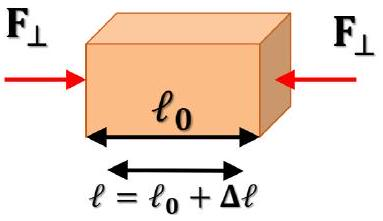
\includegraphics[max width=\textwidth, center]{2025_04_28_a9941da8947ada55c6c9g-04(1)}

Figura 3: Compresión de barra\\
Como $\ell<\ell_{0}$ entonces $\Delta \ell<0$, luego la deformación unitaria cambia de signo para evitar discrepancias entre el valor del módulo de elasticidad, por lo que $\varepsilon=-\frac{\Delta \ell}{\ell_{0}}$. La ley de Hooke se cumple para esfuerzos pequeños, luego el módulo de Young es :

$$
\begin{aligned}
Y & =\frac{\sigma}{\varepsilon} \\
& =-\frac{F_{\perp} \ell_{0}}{\Delta \ell A}
\end{aligned}
$$

Generalmente el módulo de young para tensión y compresión es el mismo(excepciones: concreto, hormigón).\\
En muchas situaciones, hay esfuerzo de compresión y tensión al mismo tiempo, generando flexión como se muestra en la figura.\\
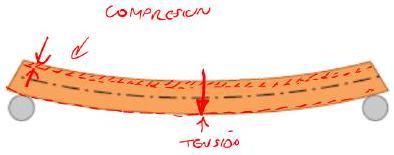
\includegraphics[max width=\textwidth, center]{2025_04_28_a9941da8947ada55c6c9g-04}

Figura 4: Barra que se pandea por su propio peso

\subsection*{2.3. Esfuerzo y deformación volumétrico}
Para un esfuerzo en forma de presión casi uniforme, que actúa en todas las direcciones sobre un objeto, ocasiona un cambio de volumen, por lo que tenemos a la deformación volumétrica unitaria( $\varepsilon_{V}$ ) y el esfuerzo volumétrico $\left(\sigma_{V}\right)$. Si un objeto se sumerge en un fluido en reposo, el fluido ejerce una fuerza sobre todas las partes de la superficie del objeto; esta fuerza es perpendicular a la superficie(si fuese paralela, el fluido se deslizaría a los lados para contrarrestar la acción). Como todo objeto está sometido a una presión inicial ( $p_{0}$ ), entonces el esfuerzo volumétrico representaría el cambio de la presión ( $\sigma_{V}=\Delta p$ ). Para el caso de compresión, tenemos:\\
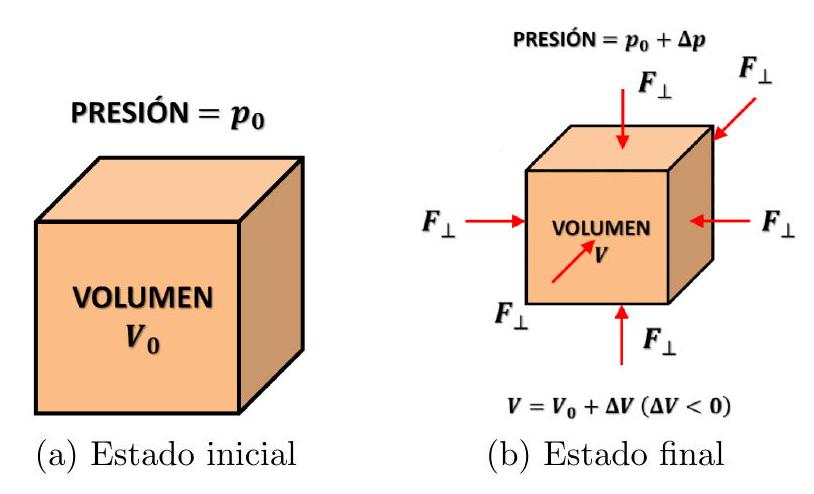
\includegraphics[max width=\textwidth, center]{2025_04_28_a9941da8947ada55c6c9g-05}

Tenemos que la deformación volumétrica unitaria es $\varepsilon_{V}=-\frac{\Delta V}{V_{0}}$. Si el cambio de presión es pequeño, entonces tenemos la ley de hooke con módulo volumétrico(B):

$$
\begin{aligned}
B & =-\frac{\sigma_{V}}{\varepsilon_{V}} \\
& =-\frac{\Delta p \cdot V_{0}}{\Delta V}
\end{aligned}
$$

\subsection*{2.4. Esfuerzo y deformación por corte}
Para una situación de esfuerzo-deformación por corte, las fuerzas no actúan de forma normal a las superficies, sino que actúan de forma tangente a la superficie. Luego tenemos al esfuerzo de corte $\sigma=\frac{F_{\|}}{A}$. Entonces el objeto presenta los siguientes estados:\\
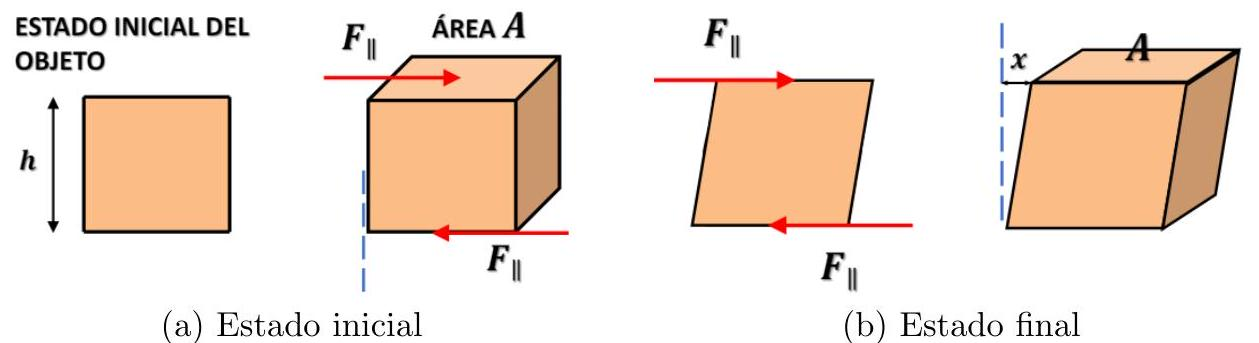
\includegraphics[max width=\textwidth, center]{2025_04_28_a9941da8947ada55c6c9g-05(1)}

Luego definimos la deformación unitaria por corte como $\varepsilon=\frac{x}{h}$. En situaciones reales\\
$x \ll h$, por lo que si las fuerzas son lo suficientemente pequeñas como para que se cumpla la ley de Hooke, entonces definimos al módulo de corte o cillazadura $(G)$ como:

$$
\begin{aligned}
G & =\frac{\sigma}{\varepsilon} \\
& =\frac{F \cdot h}{A \cdot x}
\end{aligned}
$$

Se comprueba de manera experimental y teórica que $\frac{Y}{3}<G<\frac{Y}{2}$. Tener en cuenta que estos conceptos funcionan solo para sólidos, puesto que los fluidos no tienen forma definida.

\subsection*{2.5. Deformaciones transversales}
Experimentalmente, cuando se realiza un esfuerzo de tensión, se observan deformaciones longitudinales y transversales respecto a la dirección de la fuerza. Se observa\\
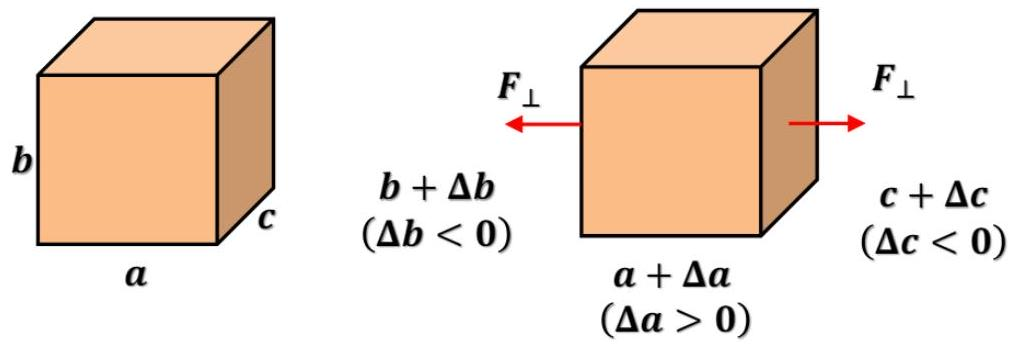
\includegraphics[max width=\textwidth, center]{2025_04_28_a9941da8947ada55c6c9g-06}

Figura 5: Objeto sometido a esfuerzo por tensión\\
que para el caso de esfuerzo por tensión, hay estiramiento longitudinal y compresiones transversales. Considerando al eje X como paralelo a la dirección de la fuerza, tenemos que el eje $Y \| b$ y el eje $Z \| c$. De esto obtenemos las deformaciones unitarias respecto a cada eje $\varepsilon_{x}=\frac{\Delta a}{a}, \varepsilon_{y}=-\frac{\Delta b}{b}$ y $\varepsilon_{z}=-\frac{\Delta c}{c}$. Considerando material isotrópico(Mismas propiedades en todas las direcciones en su interior), tenemos que $\varepsilon_{y}=\varepsilon_{z}$. Dentro de la zona elástica de un material, se tiene que la relación entre la deformación transversal unitaria y la deformación unitaria por tensión es constante(coeficiente de Poisson $\nu$ ). Luego tenemos:


\begin{equation*}
\nu=-\frac{\varepsilon_{y}}{\varepsilon_{x}} \tag{4}
\end{equation*}


Donde $\varepsilon_{y}$ es la deformación transversal y $\varepsilon_{x}$ es la deformación por tensión. Respecto a la deformación volumétrica unitaria, tomamos un elemento diferencial de dimensiones\\
$d a, d b$ y $d b$ paralelas a los ejes X, Y, Z respectivamente. Entonces tenemos:

$$
\begin{aligned}
\varepsilon & =\frac{d V}{V} \\
& =\frac{d(a b c)}{a b c} \\
& =\frac{b c d(a)+a c d(b)+a b d(c)}{a b c} \\
& =\frac{d(a)}{a}+\frac{d(b)}{b}+\frac{d(c)}{c} \\
& =\varepsilon_{x}+\varepsilon_{y}+\varepsilon_{z}
\end{aligned}
$$

Donde $\varepsilon_{x}, \varepsilon_{y} \mathrm{y} \varepsilon_{z}$ son las deformaciones unitarias totales respecto a cada eje.

\subsection*{2.5.1. Principio de superposición}
Si se cumple la ley de Hooke y se supone que los desplazamientos producidos por las fuerzas actuantes son muy pequeños en relación a las dimensiones del cuerpo, de tal manera que podamos considerar que mantiene la forma y dimensiones originales, entonces puede aplicarse el principio de superposición(los efectos que un sistema de fuerzas aplicadas origina en cuerpo son iguales a la suma de los efectos que originan estas fuerzas actuando por separado).\\
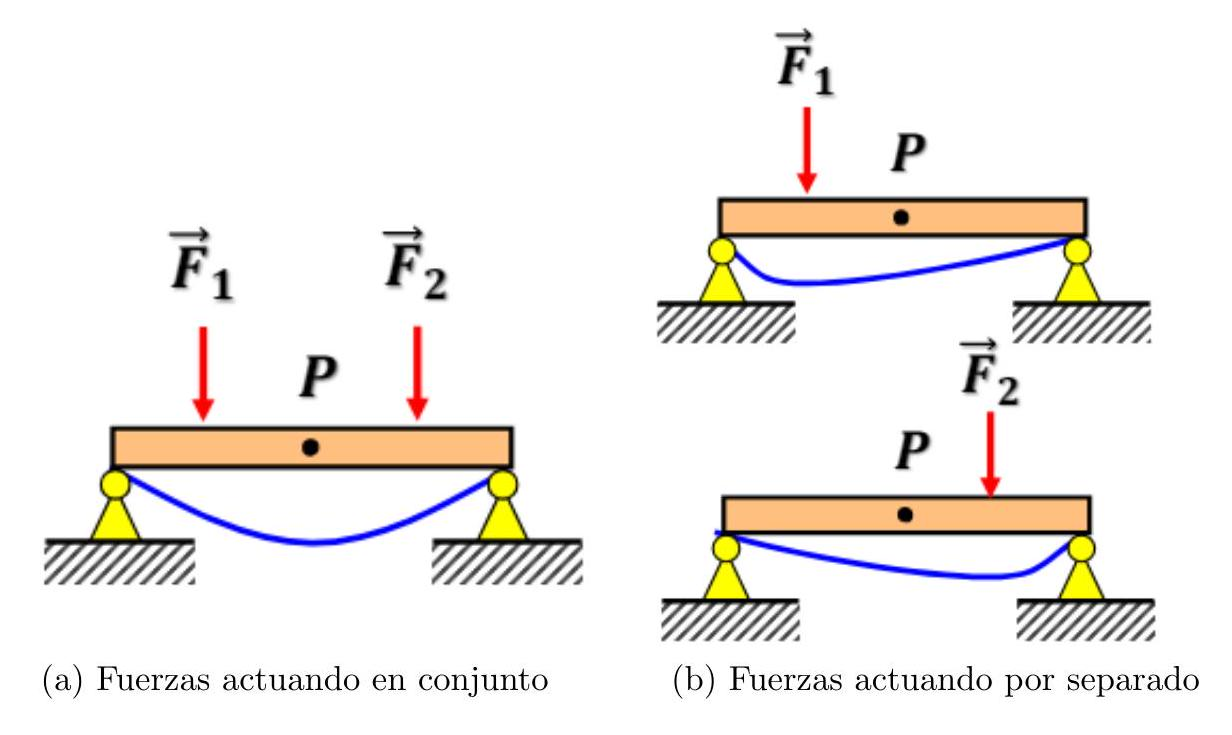
\includegraphics[max width=\textwidth, center]{2025_04_28_a9941da8947ada55c6c9g-07}

\subsection*{2.6. Elasticidad y plasticidad}
La ley de Hooke tiene un intervalo de validez. Para hallar el límite de validez, se procede a graficar el diagrama de esfuerzo-deformación. Como ejemplo, tenemos el diagrama esfuerzo-deformación típica de un metal dúctil sometido a tensión.\\
Del diagrama podemos concluir lo siguiente:\\
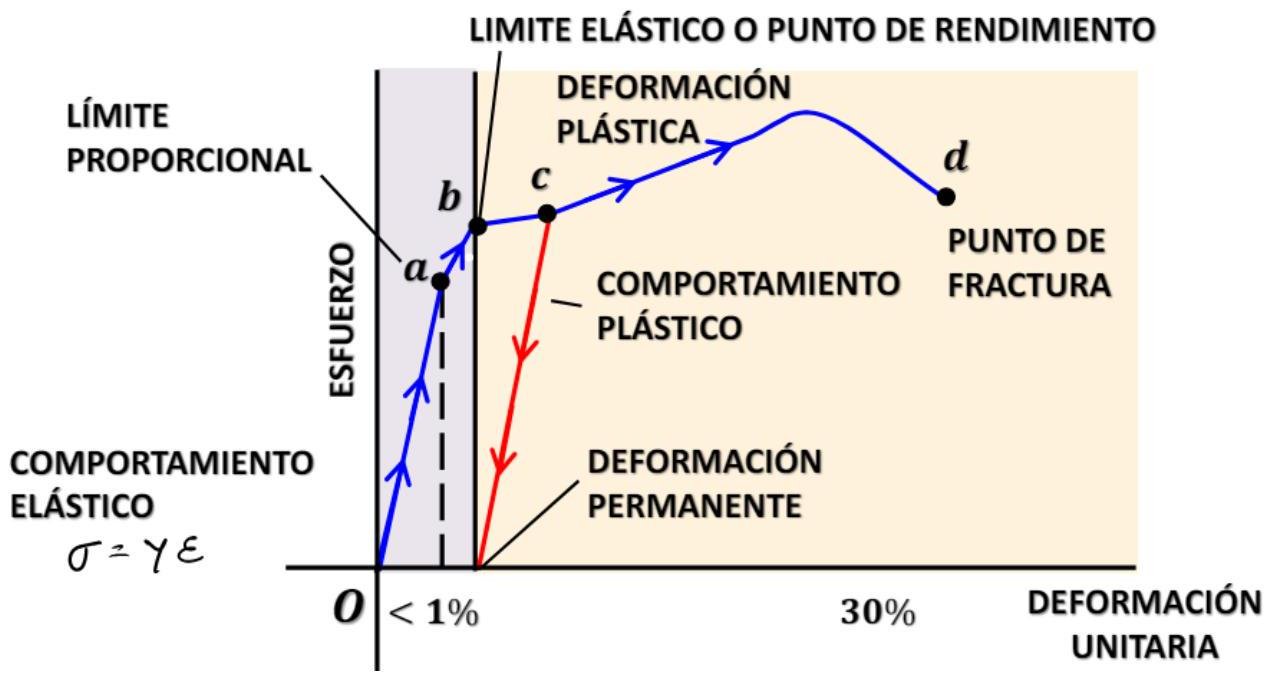
\includegraphics[max width=\textwidth, center]{2025_04_28_a9941da8947ada55c6c9g-08}

Figura 6: Diagrama esfuerzo deformación

\begin{itemize}
  \item La primera porción es una línea recta(antes de a), indicando un comportamiento acorde a la ley de Hooke.
  \item El esfuerzo en el punto a se denomina límite proporcional.
  \item Del punto a al punto b, el esfuerzo y deformación ya no son proporcionales y no se cumple la ley de Hooke, pero si la carga se retira gradualmente partiendo de cualquier punto entre O y b, se represa por la curva hasta que el material recupere su longitud original(comportamiento elástico).
  \item El esfuerzo en el punto b representa el límite elástico(o punto de rendimiento).
  \item Para un esfuerzo mayor al presente en b, se tendrá un comportamiento inelástico o plástico(el objeto no vuelve a su forma original), desplazándose por la curva hasta llegar a la parte roja y lograr deformación permanente.
  \item Para un esfuerzo más allá del presente en c, tenemos que en d se llega a la fractura.
  \item El comportamiento entre b y d se denomina flujo plástico o deformación plástica.
\end{itemize}

\subsection*{2.7. Histéresis elástica}
Para un objeto que se estira y luego se deja relajar, puede llegar a ocurrir algo muy excepcional. Tomando de ejemplo a una curva esfuerzo-deformación de caucho vulcanizado estirado a más de siete veces su longitud original, tenemos:\\
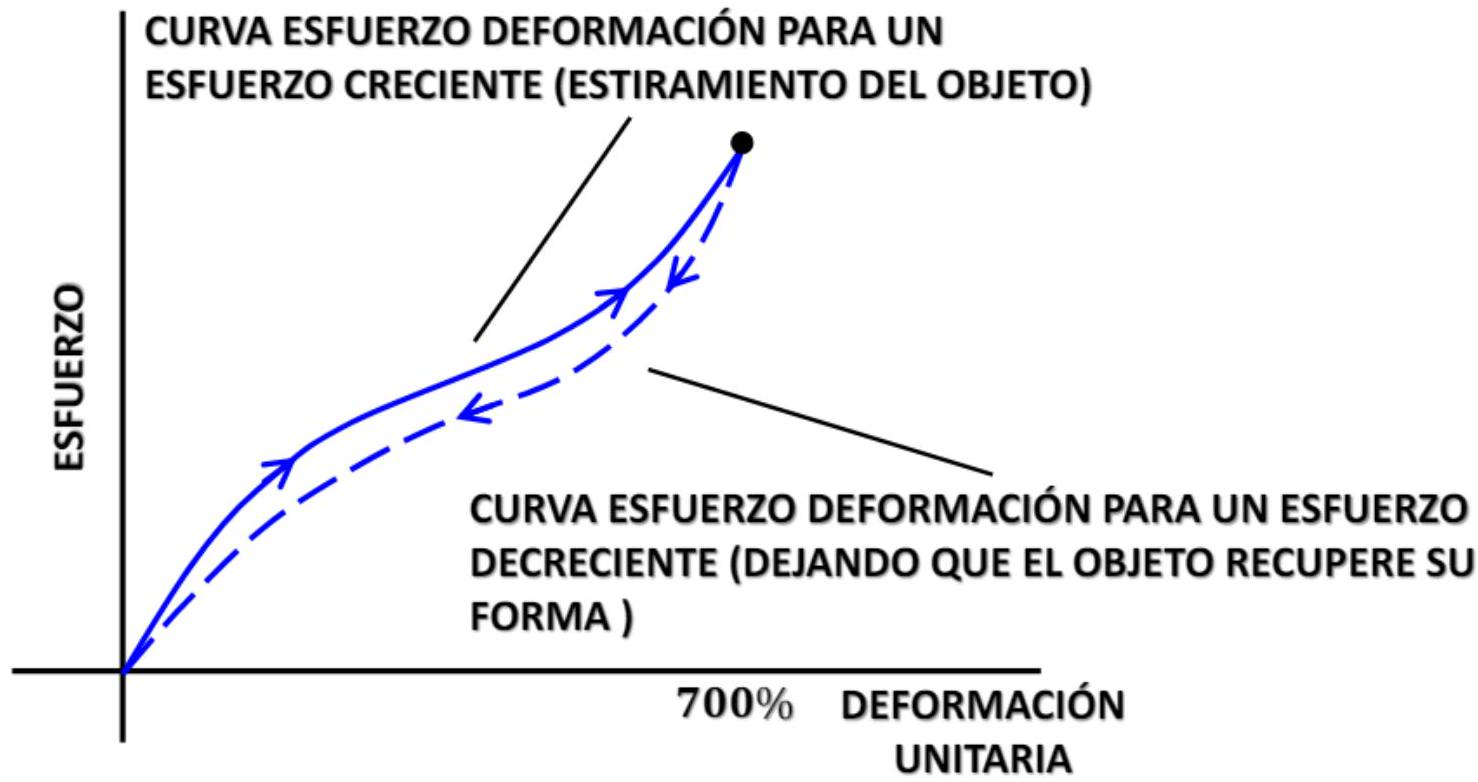
\includegraphics[max width=\textwidth, center]{2025_04_28_a9941da8947ada55c6c9g-09}

Figura 7: Diagrama esfuerzo-deformación para el caucho vulcanizado

Se observa que el esfuerzo no es proporcional a la deformación, pero el comportamiento es elástico. Se observa también que el material sigue curvas diferentes respecto a aumento y disminución del esfuerzo. Esto se denomina histéresis elástica.

\subsection*{2.8. Aplicaciones al experimento}
Para lograr el objetivo principal del experimento, se hará uso de la teoría anteriormente presentada, diferenciando el esfuerzo técnico como $\sigma_{0}=\frac{F}{S_{0}}(F$ es la fuerza perpendicular a la superficie y $S_{0}$ es el área inicial de la sección transversal del objeto) y al esfuerzo real como $\sigma=\frac{F}{S}$ ( $S$ es el área final de la sección transversal del objeto). Para el experimento, se utilizarán masas, de modo que el esfuerzo y deformación unitaria se acomoden a la ley de Hooke y halla un comportamiento elástico.

\section*{3. Equipo utilizado y diagrama de flujo del experimento}
\subsection*{3.1. Equipo utilizado}
\begin{itemize}
  \item Un resorte
  \item Una liga
  \item Cinco masas diferentes
  \item Un pie de rey
  \item Una regla milimetrada
  \item Una balanza
  \item Un soporte universal
\end{itemize}

\subsection*{3.2. Diagrama de flujo del experimento}
\begin{center}
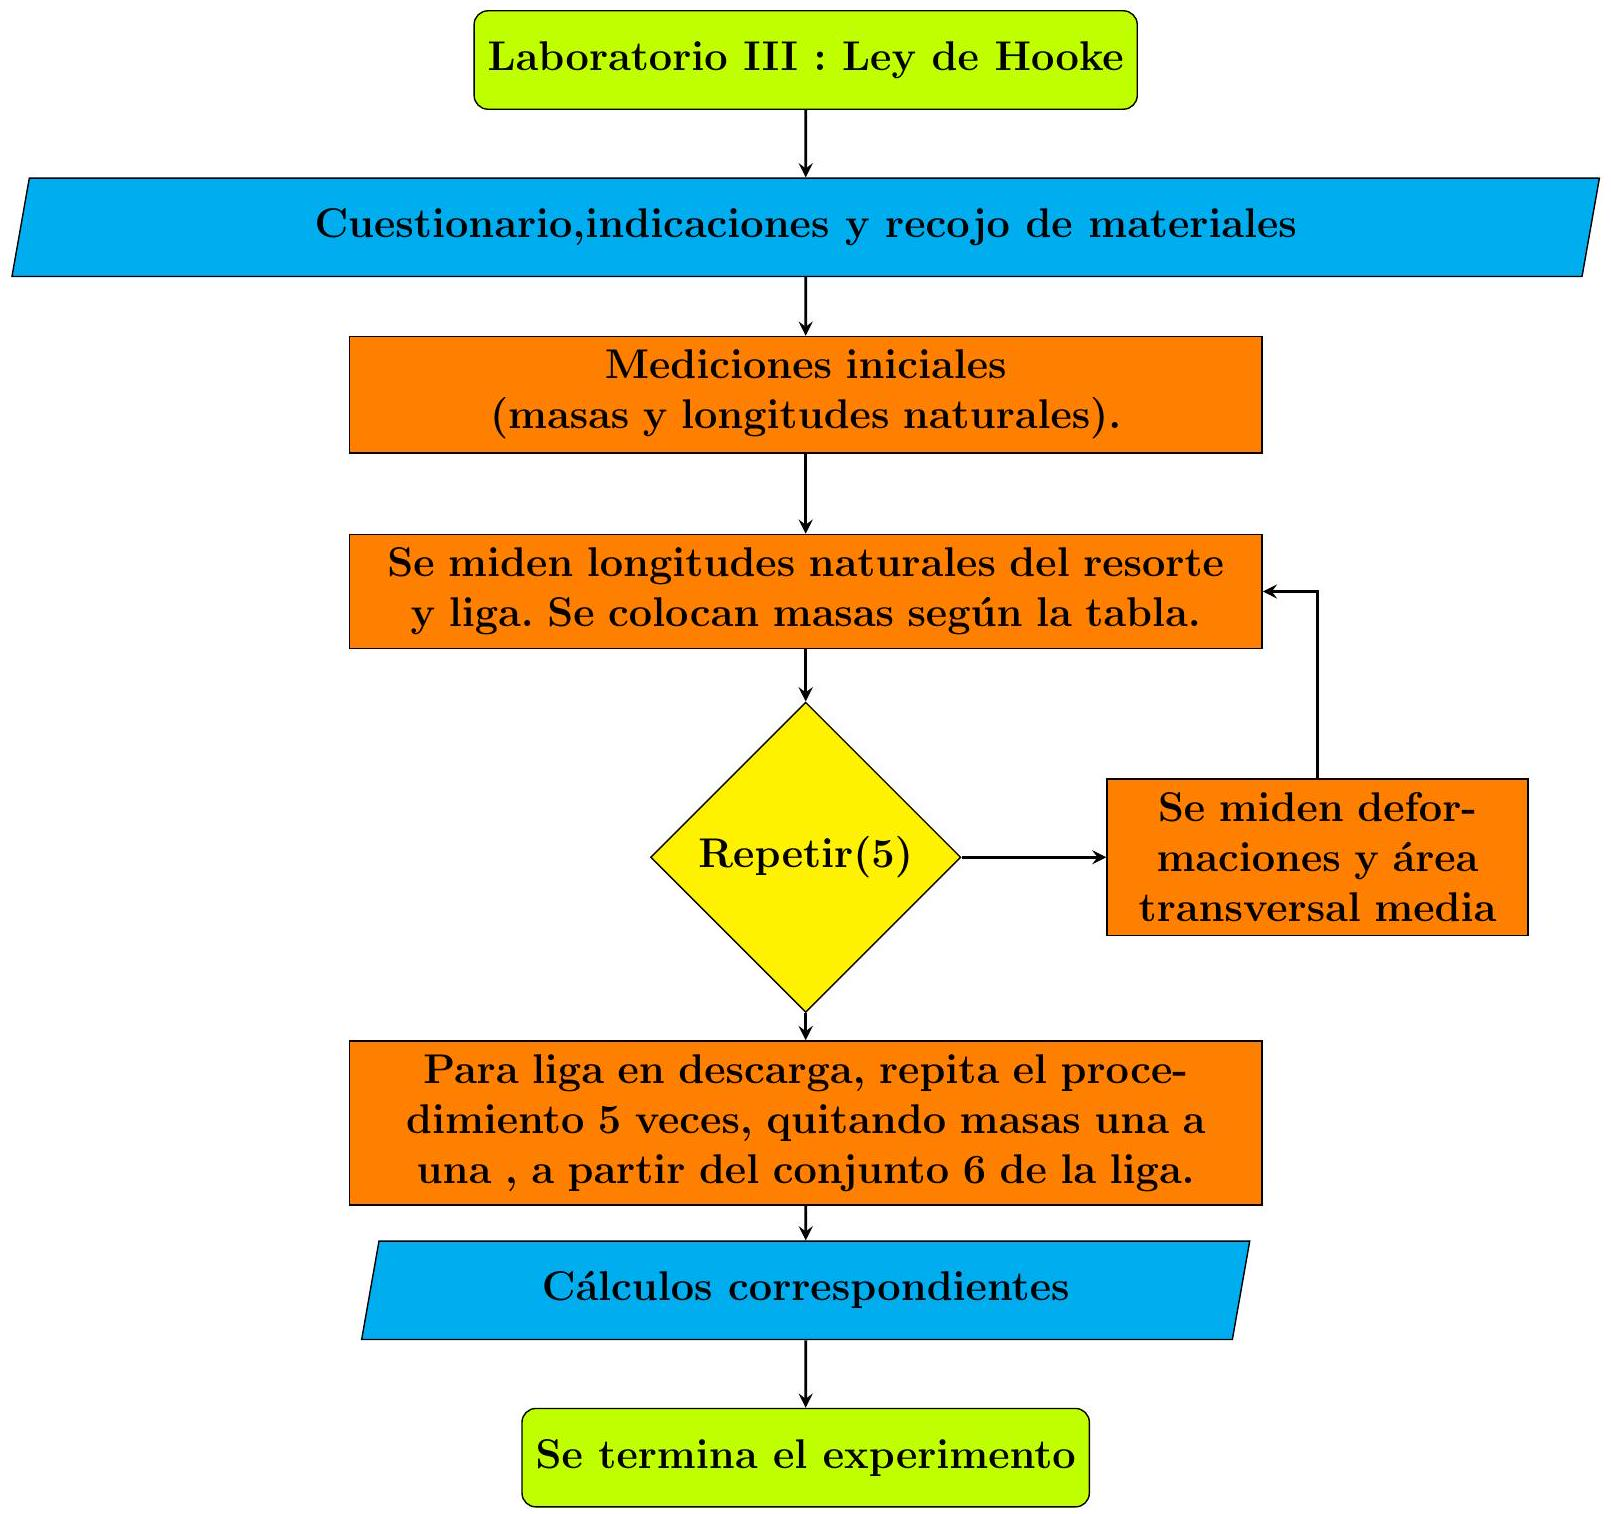
\includegraphics[max width=\textwidth]{2025_04_28_a9941da8947ada55c6c9g-10}
\end{center}

\section*{4. Procedimiento experimental}
\subsection*{4.1. Procedimiento para el resorte}
\begin{enumerate}
  \item Medir la masa del resorte, longitud natural y diámetro de la sección transversal(parte media de longitud natural).
\end{enumerate}

\begin{enumerate}
  \setcounter{enumi}{1}
  \item Colocar una masa en el extremo libre del resorte y medir la nueva longitud y diámetro de sección transversal del resorte estirado.
  \item Repetir el paso anterior para otras cuatro masas diferentes especificadas por el profesor.
\end{enumerate}

\subsection*{4.2. Procedimiento para la liga}
\begin{enumerate}
  \item Repetir el procedimiento anteriormente descrito para la liga(medir ancho, largo y nueva longitud de la liga en cada estiramiento para obtener el área de la sección transversal y la deformación).
  \item Realizar el proceso de descarga, que consiste en retirar las masas una por una, después de estirar a la liga(medir ancho, largo y nueva longitud).
\end{enumerate}

\section*{5. Cálculos y resultados}
\subsection*{5.1. Uso de unidades}
\begin{itemize}
  \item Unidad de la regla usada ( $\ell$ ): 1 cm
  \item Unidad de la balanza digital (m) : 1 g
  \item Unidad del pie de rey (p) : 1 mm
\end{itemize}

\subsection*{5.2. Uso de cifras significativas}
\begin{itemize}
  \item Se utilizan solo hasta dos cifras decimales por cada medición realizada(En sus respectivas unidades).
  \item Se utilizan hasta 4 cifras significativas en el cálculo de áreas, esfuerzos y módulos elásticos.
\end{itemize}

\subsection*{5.3. Cálculo de errores}
\begin{itemize}
  \item Error de la regla : $\Delta \ell=0,5 \mathrm{~cm}$
  \item Error de la balanza digital : $\Delta m=0,1 g$
  \item Error del pie de rey : $\Delta p=0,03 m m$
\end{itemize}

\subsection*{5.4. Resultados obtenidos y comparación con otros conocidos}
\subsection*{5.4.1. Tablas, gráficos y comparación con otros resultados conocidos}
\begin{center}
\begin{tabular}{|l|l|l|l|l|}
\hline
 & \multicolumn{2}{|r|}{Masas ( $\Delta m=0,1 \mathrm{~g}$ )} & Longitudes $(\Delta x=0,5 \mathrm{~mm})$ & Diámetro ( $\Delta D=0,03 \mathrm{~mm})$ \\
\hline
$\mathrm{N}^{\circ}$ & Nominal & $\operatorname{Real}(\mathrm{g})$ & $\mathrm{L}\left(10^{-3} \mathrm{~m}\right)$ & $\mathrm{D}\left(10^{-3} \mathrm{~m}\right)$ \\
\hline
1 & 500 & 501.0 & 227 & 13.74 \\
\hline
2 & 750 & 755.7 & 275 & 12.67 \\
\hline
3 & 1000 & 1004.6 & 317 & 11.65 \\
\hline
4 & 1250 & 1259.3 & 362 & 10.83 \\
\hline
5 & 1500 & 1505.6 & 404 & 10.51 \\
\hline
6 & 1750 & 1760.3 & 447 & 10.19 \\
\hline
\end{tabular}
\end{center}

Cuadro 1: Tabla de datos para el resorte\\
Donde $D_{0}=14 \mathrm{~mm}, m_{\text {resorte }}=59,7 \mathrm{~g}, L_{0}=191 \mathrm{~mm}$.

\begin{center}
\begin{tabular}{|l|l|l|l|l|l|}
\hline
$\mathrm{N}^{\circ}$ & Peso(N) & $\mathrm{S}\left(10^{-6} m^{2}\right)$ & $\Delta \mathrm{L}\left(10^{-3} \mathrm{~m}\right)$ & $\sigma(\mathrm{Pa})$ & $\varepsilon$ \\
\hline
1 & 4.915 & 148,273 & 36 & 33146.936 & 0.188 \\
\hline
2 & 7.413 & 126.079 & 84 & 58799.728 & 0.440 \\
\hline
3 & 9.855 & 106.596 & 126 & 92452.881 & 0.660 \\
\hline
4 & 12.354 & 92.118 & 171 & 134106.990 & 0.895 \\
\hline
5 & 14.770 & 86.755 & 213 & 170248.502 & 1.115 \\
\hline
6 & 17.269 & 81.553 & 256 & 211747.088 & 1.340 \\
\hline
\end{tabular}
\end{center}

Cuadro 2: Valores procesados de la tabla 1

\begin{center}
\begin{tabular}{|l|l|l|l|l|l|}
\hline
 & \multicolumn{2}{|r|}{Masas ( $\Delta m=0,1 \mathrm{~g}$ )} & Longitudes $(\Delta x=0,5 \mathrm{~mm})$ & \multicolumn{2}{|c|}{Dimensiones ( $\Delta a=0,03 \mathrm{~mm}$ )} \\
\hline
$\mathrm{N}^{\circ}$ & Nominal & $\operatorname{Real}(g)$ & $\mathrm{L}\left(10^{-3} m\right)$ & $\mathrm{a}\left(10^{-3} \mathrm{~m}\right)$ & $\mathrm{b}\left(10^{-3} \mathrm{~m}\right)$ \\
\hline
1 & 500 & 501.0 & 318 & 14.60 & 5.50 \\
\hline
2 & 750 & 755.7 & 334 & 14.48 & 5.44 \\
\hline
3 & 1000 & 1004.6 & 346 & 14.42 & 5.40 \\
\hline
4 & 1250 & 1259.3 & 376 & 14.32 & 5.20 \\
\hline
5 & 1500 & 1505.6 & 398 & 14.22 & 5.18 \\
\hline
6 & 1750 & 1760.3 & 426 & 14.06 & 5.04 \\
\hline
\end{tabular}
\end{center}

Cuadro 3: Datos para liga (carga)

\begin{center}
\begin{tabular}{|l|l|l|l|l|l|}
\hline
 & \multicolumn{2}{|r|}{Masas ( $\Delta m=0,1 g$ )} & Longitudes $(\Delta x=0,5 \mathrm{~mm})$ & \multicolumn{2}{|c|}{Dimensiones ( $\Delta a=0,03 \mathrm{~mm}$ )} \\
\hline
$\mathrm{N}^{\circ}$ & Nominal & $\operatorname{Real}(g)$ & $\mathrm{L}\left(10^{-3} m\right)$ & $\mathrm{a}\left(10^{-3} \mathrm{~m}\right)$ & $\mathrm{b}\left(10^{-3} \mathrm{~m}\right)$ \\
\hline
5 & 1500 & 1505.6 & 418 & 14.12 & 5.14 \\
\hline
4 & 1250 & 1259.3 & 391 & 14.40 & 5.20 \\
\hline
3 & 1000 & 1004.6 & 362 & 14.68 & 5.30 \\
\hline
2 & 750 & 755.7 & 343 & 14.72 & 5.36 \\
\hline
1 & 500 & 501.0 & 332 & 15.06 & 5.40 \\
\hline
\end{tabular}
\end{center}

Cuadro 4: Datos para liga (descarga)\\
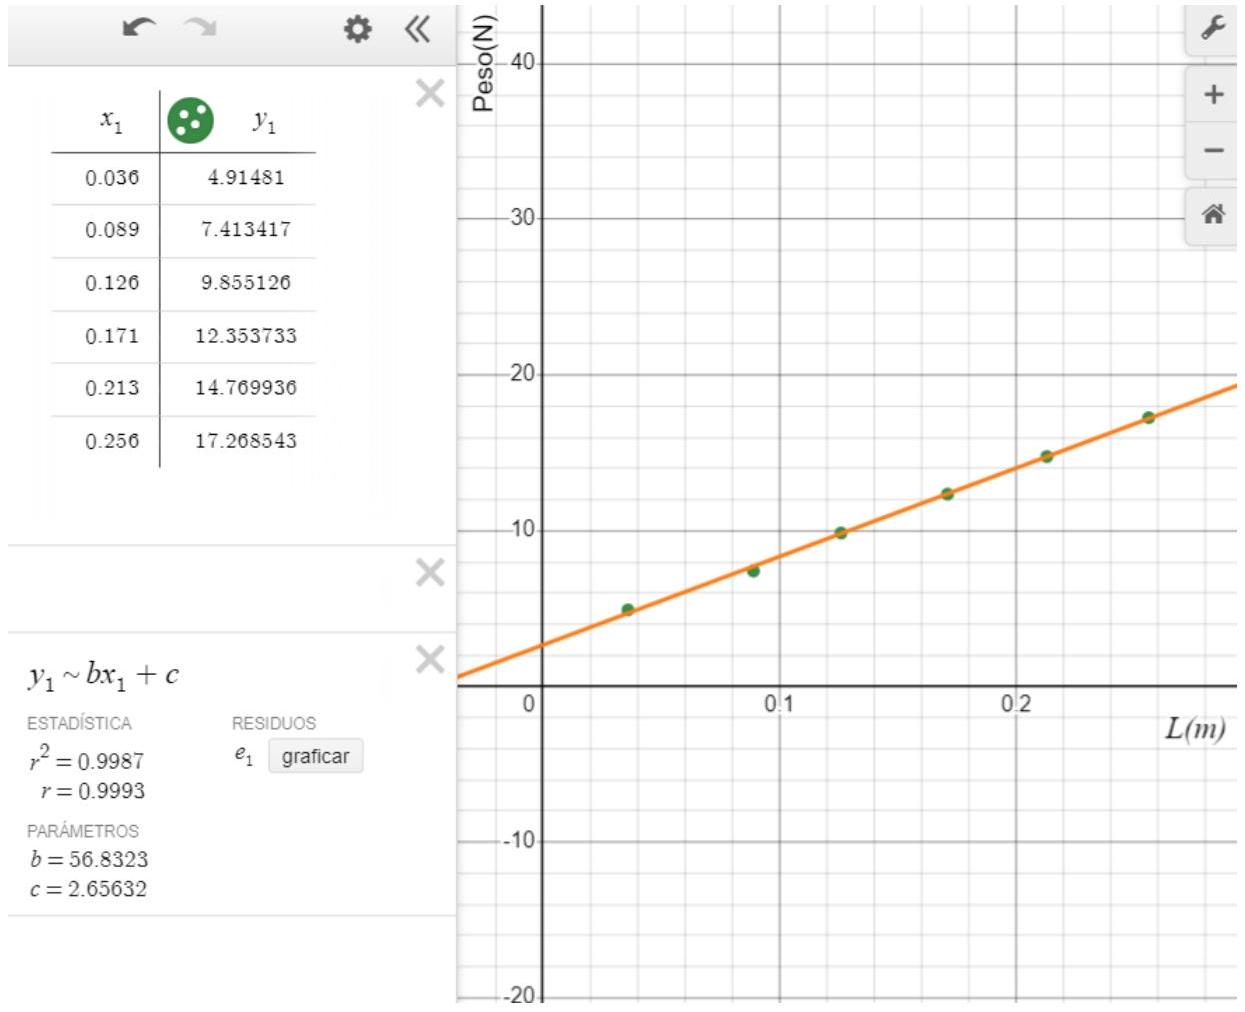
\includegraphics[max width=\textwidth, center]{2025_04_28_5f0b00b867417d4cd835g-3}

Figura 8: Gráfico F vs $\ell$

Tenemos para las tablas anteriores, que $a_{0}=15,58 \mathrm{~mm}, b_{0}=5,92 \mathrm{~mm}, m_{\text {liga }}=39,1 \mathrm{~g}$ y $L_{0}=29,6 \mathrm{~cm}$.\\
De la gráfica presente en la figura 8 , tenemos:

\begin{itemize}
  \item Se cumple la ley de Hooke(hay relación de proporcionalidad entre $F$ y $\Delta \ell$ )
  \item La constante de elasticidad viene dada por b, por lo que $k=56,8323 \frac{N}{m} \approx 56,832 \frac{N}{m}$.
  \item Se observa una precisión de 0.9987.\\
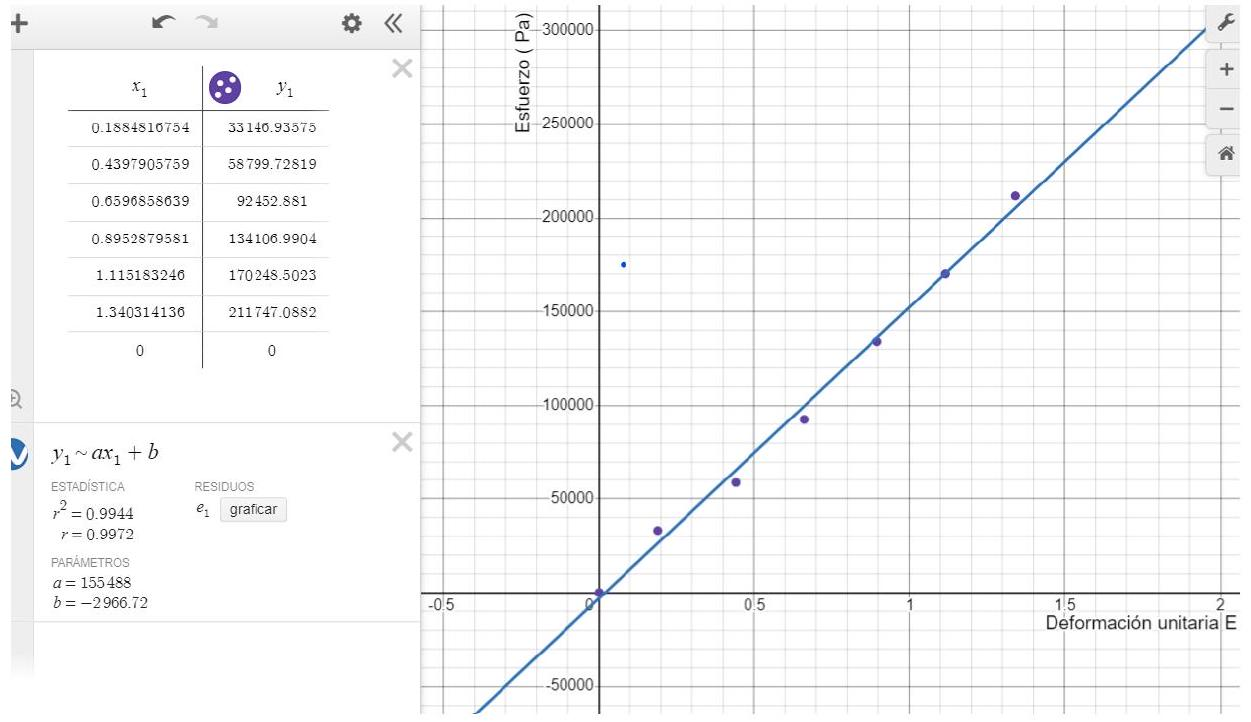
\includegraphics[max width=\textwidth, center]{2025_04_28_5f0b00b867417d4cd835g-4}
\end{itemize}

Figura 9: Gráfico $\sigma$ vs $\varepsilon$ para el resorte

De la gráfica presente en la figura 8 , tenemos:

\begin{itemize}
  \item Se observa una relación aproximada proporcional entre esfuerzo y deformación unitaria(al incluir al origen en la gráfica).
  \item De lo anterior, podemos asumir que la constante de proporcionalidad viene a ser el módulo de Young por tracción del material del resorte.
  \item Según la gráfica, el valor del módulo de Young por tracción es $Y=155488 \mathrm{~Pa}$.
\end{itemize}

Para la gráfica $\sigma$ vs $\varepsilon$ en el caso de la liga, tenemos la siguiente tabla:

\begin{center}
\begin{tabular}{|l|l|l|l|l|l|}
\hline
$\mathrm{N}^{\circ}$ & Peso(N) & $\mathrm{S}\left(10^{-6} m^{2}\right)$ & $\Delta \mathrm{L}\left(10^{-3} \mathrm{~m}\right)$ & $\sigma(\mathrm{Pa})$ & $\varepsilon$ \\
\hline
1 & 4.915 & 80.300 & 22 & 61205.604 & 0.074 \\
\hline
2 & 7.413 & 78.771 & 38 & 94113.293 & 0.128 \\
\hline
3 & 9.855 & 77.868 & 50 & 126561.951 & 0.169 \\
\hline
4 & 12.354 & 74.464 & 80 & 165902.087 & 0.270 \\
\hline
5 & 14.770 & 73.660 & 102 & 200516.104 & 0.345 \\
\hline
6 & 17.269 & 70.862 & 130 & 243691.196 & 0.439 \\
\hline
\end{tabular}
\end{center}

Cuadro 5: Valores procesados de la tabla de carga para la liga

Las incertidumbres $\Delta a$ y $\Delta D$ tienen el mismo valor de $\Delta p$ debido a que se obtuvo de mediciones con el vernier, mientras que a $\Delta(\Delta L)$ le corresponde $\Delta \ell$.

\begin{center}
\begin{tabular}{|l|l|l|l|l|l|}
\hline
$\mathrm{N}^{\circ}$ & Peso(N) & $\mathrm{S}\left(10^{-6} m^{2}\right)$ & $\Delta \mathrm{L}\left(10^{-3} \mathrm{~m}\right)$ & $\sigma(\mathrm{Pa})$ & $\varepsilon$ \\
\hline
5 & 14.770 & 72.577 & 122 & 203507.6774 & 0.412 \\
\hline
4 & 12.354 & 74.880 & 95 & 164980.409 & 0.321 \\
\hline
3 & 9.855 & 77.804 & 66 & 126666.058 & 0.223 \\
\hline
2 & 7.413 & 78.899 & 47 & 93960.611 & 0.159 \\
\hline
1 & 4.915 & 81.324 & 36 & 60434.927 & 0.122 \\
\hline
\end{tabular}
\end{center}

Cuadro 6: Valores procesados de la tabla de descarga para la liga


*Falta insertar grafica*

Figura 10: Gráfica $\sigma$ vs $\varepsilon$

De las dos tablas y el gráfico anteriores, se rescata lo siguiente:

\begin{itemize}
  \item Los esfuerzos y deformaciones unitarias por tracción son diferentes respecto a carga y descarga debido al comportamiento elástico de la liga(demora en reponerse).
  \item No hay módulo elástico ni en carga ni en descarga debido a la relación no lineal entre esfuerzo y deformación unitaria por tracción.
\end{itemize}

\section*{6. Cuestionario, observaciones y sugerencias}
\subsection*{6.1. Cuestionario}
\begin{enumerate}
  \item Llenar la tabla dada por el profesor en clase(con incertidumbres).
\end{enumerate}

R: Tablas $1,2,3$ y 4 en las páginas 12 y 13 . Se adjunta también en la parte final del documento para mantener un orden.\\
2) Para el resorte, hacer las siguientes gráficas:\\
a) Peso vs $\Delta \ell$.

R: Gráfica de la figura 8 , página 13.\\
b) $\sigma$ vs $\varepsilon$ (esfuerzo real vs deformación unitaria).

R: Gráfica de la figura 9, página 14.\\
En cada gráfico, describir la relación existente entre las magnitudes.\\
R: De la figura 8 , tenemos una relación aproximadamente proporcionalidad entre peso y deformación. De la figura 9, vemos una relación aproximadamente proporcional entre esfuerzo y deformación unitaria por tracción si añadimos el origen a la gráfica.\\
3) A partir de los gráficos, determinar(si es que hay) la constante recuperadora del resorte y el módulo de Young. Si no es posible calcularlo, explicar como se debería calcular.\\
R: De la figura 8, se puede establecer la constante elástica a partir de la pendiente de la gráfica, cuyo valor es $56,832 \frac{\mathrm{~N}}{\mathrm{~m}}$. Respecto a la figura 9 , al haber una relación aproximadamente proporcional entre esfuerzo y deformación unitaria por tensión, podemos establecer el valor del módulo de young como la pendiente de la gráfica, cuyo valor es 155488 Pa.\\
4) A partir de los gráficos de la pregunta 2 , determinar por integración numérica el trabajo realizado para producir la deformación del resorte, desde su posición de equilibrio hasta la tercera carga.\\
R: Usando regla del trapecio para la gráfica presente en la figura 8 y asumiendo que la posición de equilibrio es el origen(debido a que hay una deformación inicia por el peso del resorte), entonces tenemos los siguientes resultados:

$$
\begin{aligned}
S & \approx \sum_{i=1}^{3} \frac{\left(F\left(x_{i}\right)+F\left(x_{i-1}\right)\right)\left(x_{i}-x_{i-1}\right)}{2} \\
& =0,7824129 \mathrm{~J} \\
& \approx 0,7824 \mathrm{~J}
\end{aligned}
$$

\begin{enumerate}
  \setcounter{enumi}{4}
  \item Para el caso de la liga o del jebe, llenar la tabla correspondiente dada por el profesor para procesos de carga y descarga. Luego, representar los datos obtenidos en la gráfica $\sigma$ vs $\varepsilon$. ¿Qué representa el área encerrada por esta curva?\\
R: Gráfica presente en la figura 10 de la página 15. Para el diagrama esfuerzo deformación de la liga, tenemos que el área bajo la curva tanto para carga y descarga\\
representa la tenacidad de la liga en carga y descarga, respectivamente; la tenacidad mide la capacidad del material para absorber energía sin romperse. Por lo que, el área encerrada por las dos curvas representaría la variación de tenacidad en la liga antes y después de estirarse.
  \item Determinar de forma aproximada el área encerrada por la curva de deformaciones respecto a la liga.\\
R: Aplicando la regla del trapecio nuevamente, tenemos:
\end{enumerate}

$$
\begin{aligned}
S_{\text {descarga }} & \approx \sum_{i=1}^{6} \frac{\left(\sigma_{\text {descarga }}\left(\varepsilon_{i}\right)+\sigma_{\text {descarga }}\left(\varepsilon_{i-1}\right)\right)\left(\varepsilon_{i}-\varepsilon_{i-1}\right)}{2} \\
& =50760,8646 P a \\
S_{\text {carga }} & \approx \sum_{i=1}^{6} \frac{\left(\sigma_{\text {carga }}\left(\varepsilon_{i}\right)+\sigma_{\text {carga }}\left(\varepsilon_{i-1}\right)\right)\left(\varepsilon_{i}-\varepsilon_{i-1}\right)}{2} \\
& =60392,9971 P a \\
S_{\text {carga }}-S_{\text {descarga }} & =S_{\text {encerrada }} \approx 9632,1325 P a
\end{aligned}
$$

Luego $S_{\text {encerrada }}$ sería la variación de la tenacidad respecto a carga y descarga.\\
7) Definir esfuerzo de fluencia, esfuerzo límite, módulo de elasticidad en tracción y compresión.\\
R: El esfuerzo de fluencia representa el máximo respecto al comportamiento elástico(un esfuerzo mayor ocasiona deformaciones permanentes).\\
El esfuerzo límite representa al máximo respecto al comportamiento plástico del objeto(un esfuerzo mayor ocasiona fracturas).\\
Para esfuerzos y deformaciones unitarias de menor magnitud, se establece una relación directamente proporcional(Ley de Hooke), cuya constante de proporcionalidad viene a ser el módulo de elasticidad(tanto para tracción como para compresión, como lo explicado en el fundamento teórico, páginas 3 y 4).\\
8) ¿Qué entiende por esfuerzo normal? Explique.\\
¿Existe diferencia entre un esfuerzo tangencial y un esfuerzo de torsión?\\
R: Respecto al esfuerzo normal, viene a ser aquel producido por una fuerza perpendicular a la sección transversal del objeto(produciendo tracción o compresión).\\
El esfuerzo tangencial es aquel producido por una fuerza paralela a la superficie transversal del objeto.\\
El esfuerzo de torsión se define como la capacidad para realizar torsión de objetos en rotación alrededor de un eje fijo.\\
Se observa una clara diferencia entre esfuerzo tangencial(o cortante) y esfuerzo de torsión. El esfuerzo tangencial no genera siempre una torsión respecto al objeto, mientras que el esfuerzo de torsión es justamente la capacidad de realizar torsión en un objeto, aplicando fuerzas.

\subsection*{6.2. Observaciones}
\begin{itemize}
  \item El hecho de que solo se haya medido el diámetro de la sección transversal del resorte respecto a su mitad, no nos da una información clara respecto al esfuerzo real, debido a que las deformaciones transversales generan áreas transversales diferentes respecto a cada parte del resorte y a la liga.
  \item Respecto al diagrama esfuerzo y deformación unitaria por tracción en la liga(Figura 10), no se pudo realizar un ajuste polinomial debido a la relación entre las magnitudes respecto a los procesos de carga y descarga, por lo que se tuvo que trazar la curva a mano alzada.
  \item Durante el experimento, fue muy difícil realizar las mediciones correspondientes con el vernier, por lo que debe existir mayor incertidumbre respecto a las mediciones realizadas con esta herramienta.
  \item El hecho de que algunas de las deformaciones unitarias en la tabla 2 sean mayor a 1 , es porque se usó la longitud natural del resorte, y este superó tal longitud al poner más cargas.
  \item Respecto a la liga, esta tiene un comportamiento elástico lento respecto al tiempo transcurrido en procesos de carga y descarga.
  \item El hecho de que algunos de los esfuerzos presentes en las tablas 2,5 y 6 superen la presión atmosférica(en magnitud), es porque el área de la sección transversal del resorte y liga es mucho menor en comparación a la magnitud de la fuerza normal.
\end{itemize}

\subsection*{6.3. Sugerencias}
\begin{itemize}
  \item El vernier digital es requerido para unas mediciones con menor incertidumbre y menor dificultad.
  \item Es recomendable reponer la liga, debido a que ya se estiró bastante por múltiples experimentos anteriores.
  \item Es recomendable reponer el resorte también, debido a que este parece estar algo oxidado, perturbando su composición y por ende, el módulo de young.
\end{itemize}

\section*{7. Conclusiones}
\begin{itemize}
  \item Respecto al resorte, tenemos un comportamiento elástico debido a la relación presentada en las gráficas de las figuras 8 y 9 .
  \item Se pudo establecer una relación entre esfuerzo real y deformación unitaria por tracción, por lo que el objetivo del experimento ha sido cumplido y los valores de la constante elástica del resorte y módulo de Young han podido ser calculados.
  \item Respecto al resorte, se puede notar que la deformación unitaria es mayor en las cargas 5 y 6 de la tabla 2, por lo que la longitud final del resorte fue mayor al doble de la longitud natural del mismo.
  \item Se observa el efecto de las deformaciones transversales en el resorte, llegando a reducir el diámetro de la sección transversal del resorte. Esto quiere decir que, a mayor esfuerzo, hay mayor tracción y por lo tanto, la compresión transversal sera mayor también, reduciendo el área de la sección transversal al reducir el diámetro de esta.
  \item Respecto a la liga, se observa un comportamiento elástico muy diferente al del resorte, llegando a recuperar su forma después de un largo tiempo.
  \item Observamos en la tabla 3 y 4, los valores difieren; esto ocurre por lo mencionado en el ítem anterior.
  \item Respecto a la gráfica esfuerzo-deformación (figura 10) de la liga, podemos observar un comportamiento similar al ocurrido en la histéresis elástica.
  \item De la gráfica en la figura 10, podemos notar que los tres primeros puntos del proceso de carga parecen estar alineados(cumpliendo una relación proporcional), pero no sería certero elegir dichos puntos y conformar una zona elástica, ya que la curva de descarga no pasa por dichos puntos.
  \item El no considerar el peso de la liga y resorte fue útil para un cálculo rápido. Cabe resaltar también, que las longitudes naturales medidas incluyen a la deformación producto del peso del resorte o liga.
\end{itemize}

\section*{8. Bibliografía}
\begin{itemize}
  \item Física I , Resnick, Halliday, Krane, 341-344.
  \item Física la ciencia y tecnología Vol. I, Paul Tipler, Gene Mosca, 350-352.
\end{itemize}

\end{document}
